\documentclass[../Article_Model_Parameters.tex]{subfiles}
\graphicspath{{\subfix{../Figures/}}}
\begin{document}
	
	The present study focuses on extracting essential oil from the caraway (Carum carvi L.) seeds with supercritical fluid extraction and modelling that process. Caraway is a biennial plant belonging to the Apiaceae family. It is widespread in Asia, Europe, and North Africa. The essential oil obtained from caraway finds its potential application as a fragrance ingredient in perfumes, liquors, and toothpaste. As presented by \citet{Hromis2015}, the dried caraway contains nearly~2.8–5\% essential oil, from which the main compounds are carvone, pinene, camphene, limonene, and carveol. 
	
	The economic feasibility of the process is crucial when selecting the appropriate technology. Conventional processes, such as distillation and organic solvent extraction, are frequently used for essential oil extraction. The distillation process is carried out at a high temperature, which causes thermal degradation of thermolabile compounds—considering that alternative techniques like supercritical fluid extraction gained popularity for extraction. Supercritical carbon dioxide, in particular, is attractive due to its unique properties such as inflammable, non-toxic, low critical temperature and non-corrosive. Furthermore, its critical point is relatively low compared to other fluids, making it a suitable alternative to traditional extraction techniques. The supercritical fluids exhibit both gas- and liquid-like properties so that operating conditions can adjust the dissolving power.
	
	Various mathematical models have been proposed to describe the extraction of valuable compounds from a fixed biomass bed. However, selecting an appropriate extraction model requires understanding the physical phenomena occurring in the operational unit. Each model has its own set of assumptions and describes different mass transfer mechanisms and equilibrium relationships.
	
	One model proposed by \citet{Reverchon1993} is the hot ball model, which is based on an analogy to heat transfer and describes an extraction process from solid particles containing small quantities of solute where solubility is not a limiting factor. 
	
	Another model, the Broken-and-Intact Cell model, was presented by \citet{Sovova1994}. This model describes a system where the outer surfaces of particles have been mechanically interrupted, allowing easy access of solvent to the solute from the broken cells. In contrast, the solute from the intact cells is less accessible due to high mass transfer resistance.
	
	\citet{Reverchon1996} developed a model for fluid-solid extraction, where the oil is treated as a single component, and the extraction process is controlled by internal mass transfer resistance, neglecting external mass transfer. However, this model does not consider the influence of axial dispersion or changes in fluid density and flow rate along the bed.
	
	In this work, the fundamental governing equations are derived and combined with the kinetic model suggested by \citet{Reverchon1996} to obtain a general model for the oil extraction process from the caraway seed. This model simplifies some of the physical behaviour to obtain a control-oriented model. It is assumed that the extraction process operates semi-continuously in a cylindrical vessel. The solvent is first brought to supercritical conditions, pumped through a fixed bed of finely chopped biomass, and the solute is extracted from the biomass. The solvent and solute are then separated in a flush drum, and the extract is collected. The feed flow rate ($F_{in}$) and inlet temperature ($T_{in}$) of the extractor can be measured and manipulated, while the vessel pressure ($P$) can also be measured and manipulated. However, the outlet temperature ($T_{out}$) can only be measured. Figure \ref{fig: SFE_drawing} shows a simplified flow diagram.
	
	\begin{figure}[h!]
		\centering
		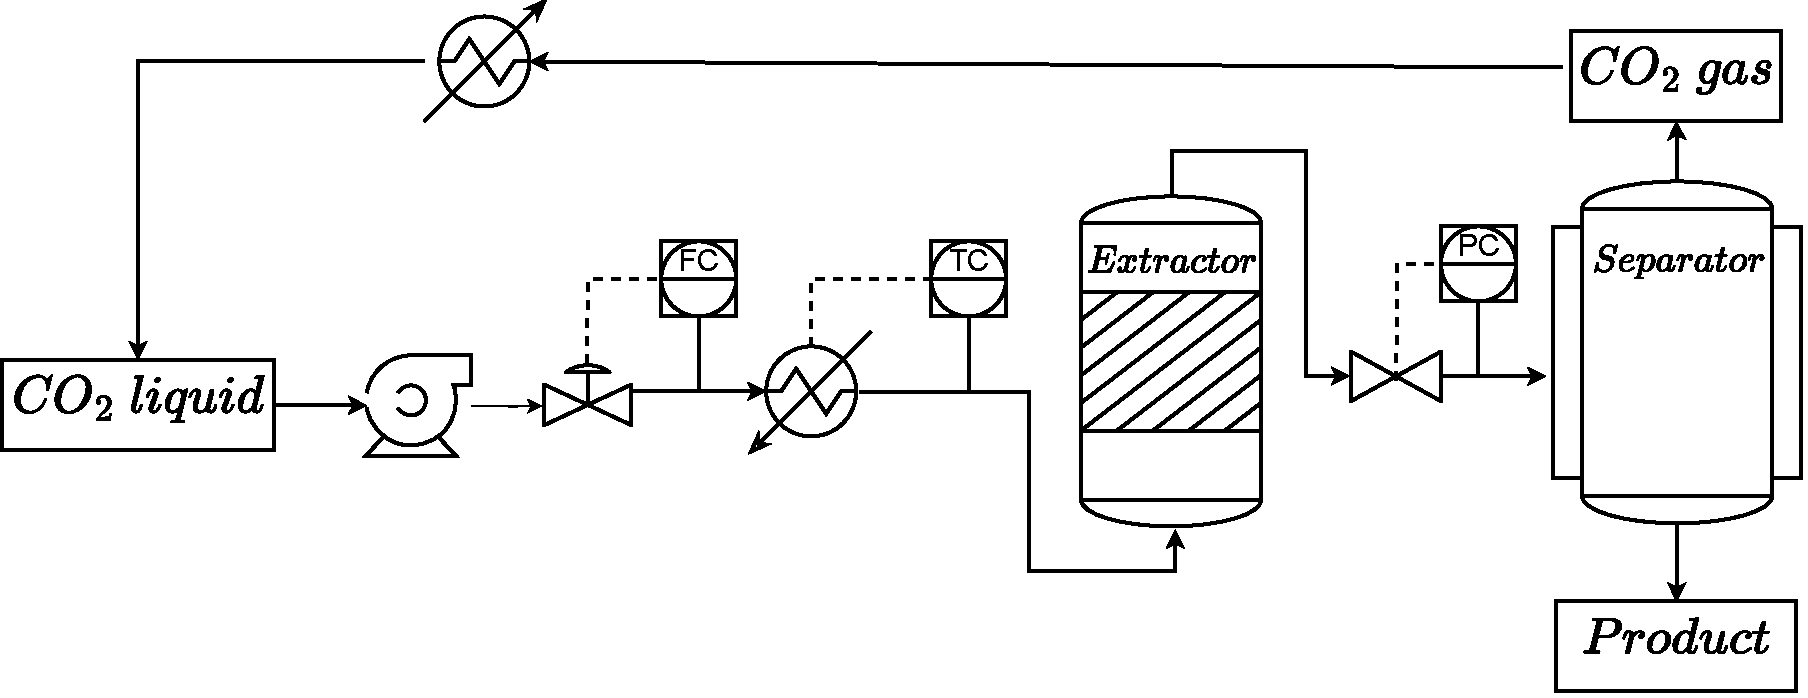
\includegraphics[width=\columnwidth]{Figures/PFD.drawio.pdf}
		\caption{Process flow diagram}
		\label{fig: SFE_drawing}
	\end{figure}

	This study aims to develop a process model for extracting natural substances from solid materials and liquids using supercritical fluids, specifically supercritical $CO_2$. To achieve this, the solvent properties are estimated based on thermodynamic relations and the extraction kinetic parameters estimated based on a set of experiments conducted at various conditions. The maximum likelihood estimator is used to solve the parameter estimation problem, and the obtained parameters are subjected to regression to derive correlations. These correlations enable the process model to be generalized across a range of temperatures (40 to $50~^\circ C$) and pressures (200 to 300 bar).
	
	The study is structured as follows: Chapter \ref{CH: Thermodynamic} provides a general discussion on supercritical fluids to familiarize the reader with their properties. Chapter \ref{CH:Governing_equations_chapter} introduces the general balance equations. The balance equations are combined with the extraction kinetic equation to develop the process model in Chapter \ref{CH: Extraction_model}. The maximum likelihood technique is presented in Chapter \ref{CH: Parameter_estimation} and is then combined with the process model. Chapter \ref{CH: Experiments} describes the experimental work and the data collected from experiments, which are used to estimate missing parameters related to the extraction kinetic. Finally, the parameter estimations and simulation results are discussed in Chapters \ref{CH: Results} and \ref{CH: Conclusion}
		
\end{document}